\documentclass{standalone}
\usepackage{tikz}
\usetikzlibrary{patterns, positioning}

\begin{document}
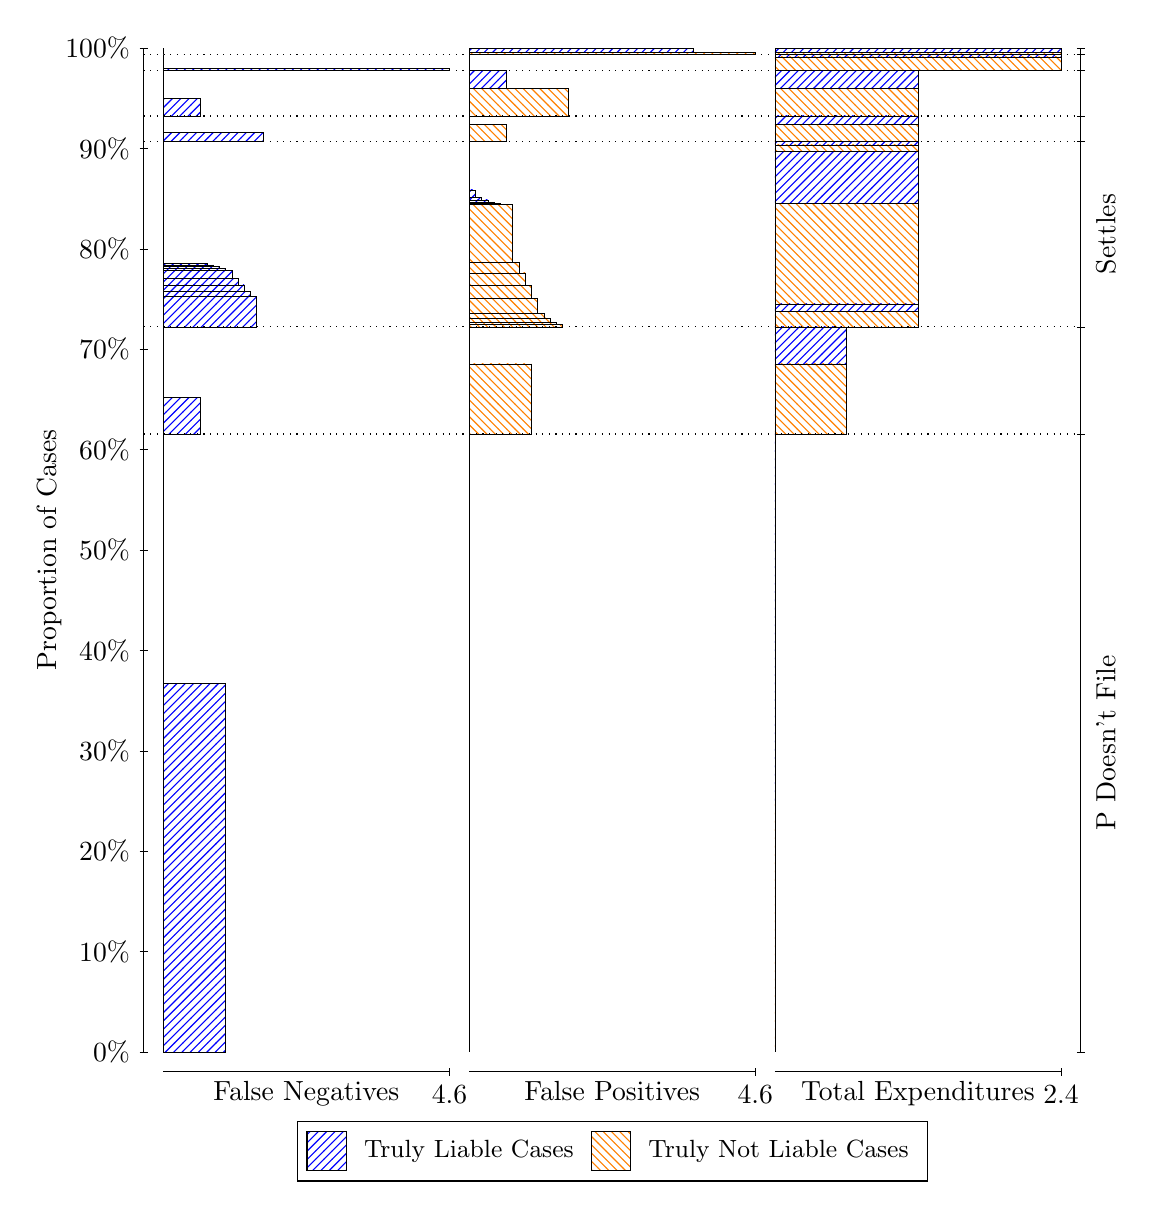
\begin{tikzpicture}
\draw[black, very thin] (1.5,1.75) -- (1.5,14.5);
\node[rotate=90, anchor=center] at (0.3, 8.125) {Proportion of Cases};
\draw[black, very thin] (1.45,1.75) -- (1.55,1.75);
\node[anchor=east] at (1.45, 1.75) {0\%};
\draw[black, very thin] (1.45,3.025) -- (1.55,3.025);
\node[anchor=east] at (1.45, 3.025) {10\%};
\draw[black, very thin] (1.45,4.3) -- (1.55,4.3);
\node[anchor=east] at (1.45, 4.3) {20\%};
\draw[black, very thin] (1.45,5.575) -- (1.55,5.575);
\node[anchor=east] at (1.45, 5.575) {30\%};
\draw[black, very thin] (1.45,6.85) -- (1.55,6.85);
\node[anchor=east] at (1.45, 6.85) {40\%};
\draw[black, very thin] (1.45,8.125) -- (1.55,8.125);
\node[anchor=east] at (1.45, 8.125) {50\%};
\draw[black, very thin] (1.45,9.4) -- (1.55,9.4);
\node[anchor=east] at (1.45, 9.4) {60\%};
\draw[black, very thin] (1.45,10.675) -- (1.55,10.675);
\node[anchor=east] at (1.45, 10.675) {70\%};
\draw[black, very thin] (1.45,11.95) -- (1.55,11.95);
\node[anchor=east] at (1.45, 11.95) {80\%};
\draw[black, very thin] (1.45,13.225) -- (1.55,13.225);
\node[anchor=east] at (1.45, 13.225) {90\%};
\draw[black, very thin] (1.45,14.5) -- (1.55,14.5);
\node[anchor=east] at (1.45, 14.5) {100\%};

\draw[black, very thin] (13.4,1.75) -- (13.4,14.5);
\draw[black, very thin] (13.35,1.75) -- (13.45,1.75);
\node[anchor=west] at (13.35, 1.75) {};
\draw[black, very thin] (13.35,9.5986) -- (13.45,9.5986);
\node[anchor=west] at (13.35, 9.5986) {};
\draw[black, very thin] (13.35,10.958) -- (13.45,10.958);
\node[anchor=west] at (13.35, 10.958) {};
\draw[black, very thin] (13.35,13.315) -- (13.45,13.315);
\node[anchor=west] at (13.35, 13.315) {};
\draw[black, very thin] (13.35,13.637) -- (13.45,13.637);
\node[anchor=west] at (13.35, 13.637) {};
\draw[black, very thin] (13.35,14.216) -- (13.45,14.216);
\node[anchor=west] at (13.35, 14.216) {};
\draw[black, very thin] (13.35,14.418) -- (13.45,14.418);
\node[anchor=west] at (13.35, 14.418) {};
\draw[black, very thin] (13.35,14.5) -- (13.45,14.5);
\node[anchor=west] at (13.35, 14.5) {};

\draw[black, very thin, pattern color=blue, pattern=north east lines] (1.75,1.75) rectangle (2.5399,6.435);
\draw[black, very thin, pattern color=orange, pattern=north west lines] (1.75,6.435) rectangle (1.75,9.5986);
\draw[black, very thin, pattern color=blue, pattern=north east lines] (1.75,9.5986) rectangle (2.2239,10.067);
\draw[black, very thin, pattern color=orange, pattern=north west lines] (1.75,10.067) rectangle (1.75,10.958);
\draw[black, very thin, pattern color=blue, pattern=north east lines] (1.75,10.958) rectangle (2.9348,11.344);
\draw[black, very thin, pattern color=blue, pattern=north east lines] (1.75,11.344) rectangle (2.8558,11.411);
\draw[black, very thin, pattern color=blue, pattern=north east lines] (1.75,11.411) rectangle (2.7768,11.493);
\draw[black, very thin, pattern color=blue, pattern=north east lines] (1.75,11.493) rectangle (2.6978,11.576);
\draw[black, very thin, pattern color=blue, pattern=north east lines] (1.75,11.576) rectangle (2.6188,11.674);
\draw[black, very thin, pattern color=blue, pattern=north east lines] (1.75,11.674) rectangle (2.5399,11.702);
\draw[black, very thin, pattern color=blue, pattern=north east lines] (1.75,11.702) rectangle (2.4609,11.731);
\draw[black, very thin, pattern color=blue, pattern=north east lines] (1.75,11.731) rectangle (2.3819,11.747);
\draw[black, very thin, pattern color=blue, pattern=north east lines] (1.75,11.747) rectangle (2.3029,11.762);
\draw[black, very thin, pattern color=orange, pattern=north west lines] (1.75,11.762) rectangle (1.75,13.315);
\draw[black, very thin, pattern color=blue, pattern=north east lines] (1.75,13.315) rectangle (3.0138,13.425);
\draw[black, very thin, pattern color=orange, pattern=north west lines] (1.75,13.425) rectangle (1.75,13.637);
\draw[black, very thin, pattern color=blue, pattern=north east lines] (1.75,13.637) rectangle (2.2239,13.863);
\draw[black, very thin, pattern color=orange, pattern=north west lines] (1.75,13.863) rectangle (1.75,14.216);
\draw[black, very thin, pattern color=blue, pattern=north east lines] (1.75,14.216) rectangle (5.3833,14.246);
\draw[black, very thin, pattern color=orange, pattern=north west lines] (1.75,14.246) rectangle (1.75,14.418);
\draw[black, very thin, pattern color=orange, pattern=north west lines] (1.75,14.418) rectangle (1.75,14.447);
\draw[black, very thin, pattern color=blue, pattern=north east lines] (1.75,14.447) rectangle (1.75,14.5);
\draw[black, very thin, pattern color=orange, pattern=north west lines] (5.6333,1.75) rectangle (5.6333,4.9136);
\draw[black, very thin, pattern color=blue, pattern=north east lines] (5.6333,4.9136) rectangle (5.6333,9.5986);
\draw[black, very thin, pattern color=orange, pattern=north west lines] (5.6333,9.5986) rectangle (6.4232,10.49);
\draw[black, very thin, pattern color=blue, pattern=north east lines] (5.6333,10.49) rectangle (5.6333,10.958);
\draw[black, very thin, pattern color=orange, pattern=north west lines] (5.6333,10.958) rectangle (6.8181,10.986);
\draw[black, very thin, pattern color=orange, pattern=north west lines] (5.6333,10.986) rectangle (6.7391,11.015);
\draw[black, very thin, pattern color=orange, pattern=north west lines] (5.6333,11.015) rectangle (6.6601,11.073);
\draw[black, very thin, pattern color=orange, pattern=north west lines] (5.6333,11.073) rectangle (6.5812,11.129);
\draw[black, very thin, pattern color=orange, pattern=north west lines] (5.6333,11.129) rectangle (6.5022,11.322);
\draw[black, very thin, pattern color=orange, pattern=north west lines] (5.6333,11.322) rectangle (6.4232,11.485);
\draw[black, very thin, pattern color=orange, pattern=north west lines] (5.6333,11.485) rectangle (6.3442,11.645);
\draw[black, very thin, pattern color=orange, pattern=north west lines] (5.6333,11.645) rectangle (6.2652,11.777);
\draw[black, very thin, pattern color=orange, pattern=north west lines] (5.6333,11.777) rectangle (6.1862,12.512);
\draw[black, very thin, pattern color=blue, pattern=north east lines] (5.6333,12.512) rectangle (6.0283,12.527);
\draw[black, very thin, pattern color=blue, pattern=north east lines] (5.6333,12.527) rectangle (5.9493,12.542);
\draw[black, very thin, pattern color=blue, pattern=north east lines] (5.6333,12.542) rectangle (5.8703,12.572);
\draw[black, very thin, pattern color=blue, pattern=north east lines] (5.6333,12.572) rectangle (5.7913,12.6);
\draw[black, very thin, pattern color=blue, pattern=north east lines] (5.6333,12.6) rectangle (5.7123,12.698);
\draw[black, very thin, pattern color=blue, pattern=north east lines] (5.6333,12.698) rectangle (5.6333,13.315);
\draw[black, very thin, pattern color=orange, pattern=north west lines] (5.6333,13.315) rectangle (6.1072,13.528);
\draw[black, very thin, pattern color=blue, pattern=north east lines] (5.6333,13.528) rectangle (5.6333,13.637);
\draw[black, very thin, pattern color=orange, pattern=north west lines] (5.6333,13.637) rectangle (6.8971,13.99);
\draw[black, very thin, pattern color=blue, pattern=north east lines] (5.6333,13.99) rectangle (6.1072,14.216);
\draw[black, very thin, pattern color=orange, pattern=north west lines] (5.6333,14.216) rectangle (5.6333,14.388);
\draw[black, very thin, pattern color=blue, pattern=north east lines] (5.6333,14.388) rectangle (5.6333,14.418);
\draw[black, very thin, pattern color=orange, pattern=north west lines] (5.6333,14.418) rectangle (9.2667,14.447);
\draw[black, very thin, pattern color=blue, pattern=north east lines] (5.6333,14.447) rectangle (8.4768,14.5);
\draw[black, very thin, pattern color=orange, pattern=north west lines] (9.5167,1.75) rectangle (9.5167,4.9136);
\draw[black, very thin, pattern color=blue, pattern=north east lines] (9.5167,4.9136) rectangle (9.5167,9.5986);
\draw[black, very thin, pattern color=orange, pattern=north west lines] (9.5167,9.5986) rectangle (10.425,10.49);
\draw[black, very thin, pattern color=blue, pattern=north east lines] (9.5167,10.49) rectangle (10.425,10.958);
\draw[black, very thin, pattern color=orange, pattern=north west lines] (9.5167,10.958) rectangle (11.333,11.152);
\draw[black, very thin, pattern color=blue, pattern=north east lines] (9.5167,11.152) rectangle (11.333,11.25);
\draw[black, very thin, pattern color=orange, pattern=north west lines] (9.5167,11.25) rectangle (11.333,12.524);
\draw[black, very thin, pattern color=blue, pattern=north east lines] (9.5167,12.524) rectangle (11.333,13.184);
\draw[black, very thin, pattern color=orange, pattern=north west lines] (9.5167,13.184) rectangle (11.333,13.271);
\draw[black, very thin, pattern color=blue, pattern=north east lines] (9.5167,13.271) rectangle (11.333,13.315);
\draw[black, very thin, pattern color=orange, pattern=north west lines] (9.5167,13.315) rectangle (11.333,13.528);
\draw[black, very thin, pattern color=blue, pattern=north east lines] (9.5167,13.528) rectangle (11.333,13.637);
\draw[black, very thin, pattern color=orange, pattern=north west lines] (9.5167,13.637) rectangle (11.333,13.99);
\draw[black, very thin, pattern color=blue, pattern=north east lines] (9.5167,13.99) rectangle (11.333,14.216);
\draw[black, very thin, pattern color=orange, pattern=north west lines] (9.5167,14.216) rectangle (13.15,14.388);
\draw[black, very thin, pattern color=blue, pattern=north east lines] (9.5167,14.388) rectangle (13.15,14.418);
\draw[black, very thin, pattern color=orange, pattern=north west lines] (9.5167,14.418) rectangle (13.15,14.447);
\draw[black, very thin, pattern color=blue, pattern=north east lines] (9.5167,14.447) rectangle (13.15,14.5);
\draw[black, dotted] (1.5,9.5986) -- (13.4,9.5986);
\draw[black, dotted] (1.5,10.958) -- (13.4,10.958);
\draw[black, dotted] (1.5,13.315) -- (13.4,13.315);
\draw[black, dotted] (1.5,13.637) -- (13.4,13.637);
\draw[black, dotted] (1.5,14.216) -- (13.4,14.216);
\draw[black, dotted] (1.5,14.418) -- (13.4,14.418);
\draw[black, very thin] (1.75,1.5) -- (5.3833,1.5);
\node[anchor=north] at (3.5667, 1.5) {False Negatives};
\draw[black, very thin] (5.3833,1.45) -- (5.3833,1.55);
\node[anchor=north] at (5.3833, 1.45) {4.6};

\draw[black, very thin] (5.6333,1.5) -- (9.2667,1.5);
\node[anchor=north] at (7.45, 1.5) {False Positives};
\draw[black, very thin] (9.2667,1.45) -- (9.2667,1.55);
\node[anchor=north] at (9.2667, 1.45) {4.6};

\draw[black, very thin] (9.5167,1.5) -- (13.15,1.5);
\node[anchor=north] at (11.333, 1.5) {Total Expenditures};
\draw[black, very thin] (13.15,1.45) -- (13.15,1.55);
\node[anchor=north] at (13.15, 1.45) {2.4};

\node[black, centered, rotate=90] at (13.72, 5.6743) {P Doesn't File};

\node[black, centered, rotate=90] at (13.72, 12.137) {Settles};





\draw (7.449999999999999,1.5) node[draw=none] (baseCoordinate) {};
\begin{scope}[align=center]
        \matrix[scale=0.5, draw=black, below=0.5cm of baseCoordinate, nodes={draw}, column sep=0.1cm]{
            \node[rectangle, draw, minimum width=0.5cm, minimum height=0.5cm, pattern=north east lines, pattern color=blue] {}; &
            \node[draw=none, font=\small] (B) {Truly Liable Cases}; &
            \node[rectangle, draw, minimum width=0.5cm, minimum height=0.5cm, pattern=north west lines, pattern color=orange] {}; &
            \node[draw=none, font=\small] (B) {Truly Not Liable Cases}; \\
            };
\end{scope}

\end{tikzpicture}
\end{document}